\documentclass[12pt,a4paper]{article}
\usepackage[utf8]{inputenc}
\usepackage[russian]{babel}
\usepackage{amsmath}
\usepackage{amssymb}
\usepackage{graphicx}
\usepackage{geometry}
\usepackage{indentfirst}
\usepackage{setspace}
\usepackage{fancyhdr}
\usepackage{booktabs}
\usepackage{array}

\geometry{left=2.5cm, right=2cm, top=2.5cm, bottom=2.5cm}
\setlength{\parindent}{1.25cm}
\onehalfspacing

\pagestyle{fancy}
\fancyhf{}
\fancyhead[C]{\thepage}
\renewcommand{\headrulewidth}{0pt}

\begin{document}

%--- Титульная страница ---
\begin{titlepage}
\begin{flushright}
{\small МЕЖОТРАСЛЕВОЙ НАУЧНО-ТЕХНИЧЕСКИЙ ЦЕНТР\\
ВЕНЧУРНЫХ НЕТРАДИЦИОННЫХ ТЕХНОЛОГИЙ}
\end{flushright}

\vspace{2cm}
\begin{flushleft}
{\small Жвирблис В.Е. Феноменологическое описание и экспериментальное
исследование некоторых кольцаров. Препринт № 33 МНЦ «ВЕНТ».
М., 1993, 38~с.

\medskip
28~илл., библ. 11~сс.}
\end{flushleft}

\vspace{1cm}
\begin{flushleft}
{\small Показано, что кольцары \textbf{жидкостей} представляют особый класс
неквантовых систем с двумя стационарными состояниями. Подробно описаны
эксперименты по изучению свойств электрофизического кольцара
и высказаны предположения о возможностях его практического использования.}

\medskip
{\small Рукопись поступила в редакцию 25.12.92~г.}
\end{flushleft}

\vfill
\begin{flushleft}
{\small © В.Е.Жвирблис, 1993\\
© МНЦ «ВЕНТ», 1993}
\end{flushleft}

\hfill
\begin{minipage}{0.45\textwidth}
\begin{flushright}
{\large Препринт № 33}

\bigskip
{\large \textbf{В.Е.Жвирблис}}

\bigskip
Феноменологическое описание и\\
экспериментальное исследование\\
некоторых кольцаров

\vspace{2cm}
{\small Москва\\
1993}
\end{flushright}
\end{minipage}
\end{titlepage}

%--- Страница 3 ---
\setcounter{page}{3}

\section*{ВВЕДЕНИЕ}

В предыдущей работе~[1] было показано, что наблюдаемая М.Ф.Лазаревым
непрерывная циркуляция летучей жидкости в замкнутом кольцеобразном сосуде
с пористой перегородкой (т.н. кольцаре), формально похожая на непрерывную
циркуляцию тока по сверхпроводящему кольцу, не является экспериментальным
артефактом и не требует кардинальной ревизии законов термодинамики, а
представляет собой следствие принципиального отличия любой реальной
термодинамической системы (т.е. системы, имеющей неравновесную метастабильную
структуру) от идеальной бесструктурной системы, находящейся в состоянии,
близком к истинному термодинамическому равновесию.

Как известно, в системах, далёких от состояния термодинамического
равновесия, могут происходить процессы самопроизвольной самоорганизации,
приводящие к возникновению т.н. диссипативных структур, типичными
представителями которых могут служить любые объекты живой природы~[2]. В
этом смысле кольцар Лазарева следует рассматривать как простую модель,
позволяющую в чистом виде наблюдать движущую силу подобных процессов. И
если такая «сила» действительно существует как физическая реальность, то
кольцар Лазарева должен быть не единственно возможным устройством подобного
рода, а лишь одним из представителей по-видимому обширного класса динамических
диссипативных структур, т.е. метастабильных структур, в которых вследствие
кинетических затруднений неопределённо долго сохраняются следы процессов,
инициировавшего их первоначальное возникновение.

Настоящая работа посвящена описанию и экспериментальному исследованию
некоторых простейших кольцаров. Полученные результаты позволяют утверждать,
что эффект, обнаруженный Лазаревым, нуждается в углублённом изучении,
поскольку его объяснение выходит далеко за пределы элементарной физики и
затрагивает проблемы весьма фундаментального характера. В частности,
обнаружение корреляции между флуктуациями мощности, развиваемой кольцарами,
и вариациями солнечной активности [ср. 3,~4], позволяет утверждать, что в
природе вообще не существует истинно изолированных систем и что поэтому
движущая сила любых процессов самоорганизации имеет в конечном счёте
космофизическое происхождение.

%--- Страница 4--5 ---
\newpage
\section*{ГЛАВА I}
\subsection*{Кольцар Лазарева}

\subsubsection*{§1. Первые наблюдения}

Один из самых информативных экспериментов Лазарева заключался в следующем.
В верхнюю часть замкнутого кольцеобразного сосуда с керамической пористой
перегородкой (рис.~1) помещалось некоторое количество воды и затем на
протяжении длительного времени (около четырёх лет) наблюдалась динамика её
подъёма в обводной трубке.

Несложный расчёт показывает, что из-за существования сил поверхностного
натяжения, действующих в капиллярах пористой перегородки, жидкость в обводной
трубке должна подниматься не до уровня $H_2 - H_1$, а до уровня
\[
H' = H_2 - H_1 + \frac{2\sigma\cos\theta}{\rho g z},
\]
где $\sigma$ — поверхностное натяжение, $\theta$ — краевой угол, $\rho$ —
плотность жидкости, $z$ — радиус капилляров пористой перегородки, а $g$ —
ускорение свободного падения. При этом, естественно, предполагается, что
система находится в строго изотермических условиях.

Именно такой дополнительный подъём жидкости, вызванный силами капиллярного
давления и хорошо согласующийся с расчётом, и наблюдал Лазарев в одном из
экспериментов (рис.~2). На графике отчётливо видны три стадии процесса:
быстрое достижение баланса сил гидростатического давления (излом на уровне
$H_2 - H_1$), значительно более медленный подъём уровня жидкости в обводной
трубке вследствие действия сил капиллярного давления вплоть до достижения
полного баланса всех сил (излом на уровне $H'$) и, наконец, длительная
квазистационарная стадия, когда в системе не происходило никаких заметных
изменений.

\begin{figure}[h]
\centering
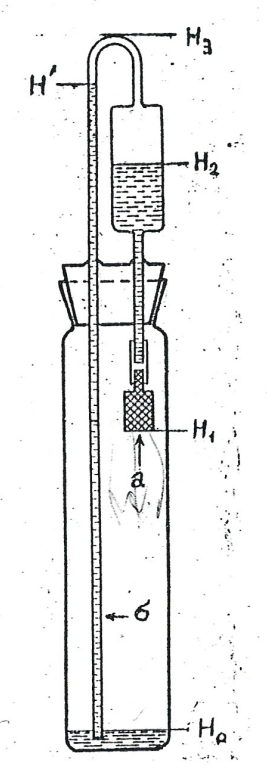
\includegraphics[width=0.3\textwidth]{fig_01.png}
\caption*{\textbf{Рис. 1.} Схема кольцара Лазарева: а~— пористая перегородка,
б~— обводная трубка}
\end{figure}

Таким образом, совершенно очевидно, что уровень воды (или какой-либо другой
жидкости) может устойчиво превышать уровень в пространстве над пористой
перегородкой при выполнении простого условия
\begin{equation}
\frac{2\sigma\cos\theta}{\rho g z} > H_1,
\end{equation}
соблюдённого в описанном выше эксперименте Лазарева. Точно так же совершенно
очевидно, что эта квазистационарная стадия не может длиться бесконечно долго:
система в принципе неравновесна, и жидкость, находящаяся над пористой
перегородкой, либо рано или поздно переместится вниз. Вопрос заключается
только в том, как скоро и каким образом это может произойти.

По-видимому, мы имеем дело с каким-то очень медленным процессом, поскольку
Лазарев не наблюдал заметных изменений уровня $H'$ на протяжении четырёх лет.
Таким процессом может служить изотермическая переконденсация, происходящая
вследствие различия давлений насыщенного пара жидкости в поле тяготения на
уровне $H_0$, условно принятом за нулевой, и на высоте $H_1$.

\begin{figure}[h]
\centering
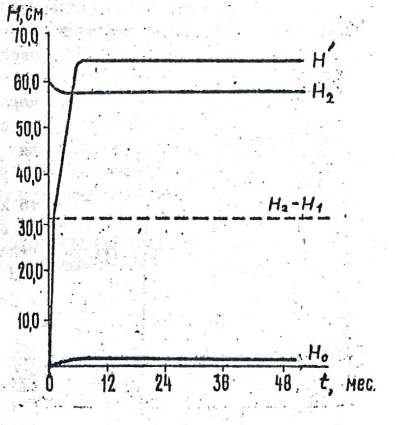
\includegraphics[width=0.45\textwidth]{fig_02.png}
\caption*{\textbf{Рис. 2.} Результат одного из экспериментов Лазарева}
\end{figure}

Если давление насыщенного пара непосредственно над её поверхностью равно
$P_0$, то на высоте $H$ его давление определяется т.н. барометрической формулой
\[
P_H = P_0\, e^{-\frac{m_\text{м} g H}{kT}},
\]
где $m_\text{м}$ — масса молекулы жидкости, $k$ — постоянная Больцмана, а
$T$ — абсолютная температура. Поэтому в установке, изображённой на рис.~1,
жидкость будет самопроизвольно испаряться с поверхности пористой перегородки
и конденсироваться на дне сосуда. В результате этого уровни $H_2$ и $H'$
станут очень медленно понижаться, причём между ними будет сохраняться разность
\[
\Delta H = \frac{2\sigma\cos\theta}{\rho g z} - H_1.
\]
А после того, как над пористой перегородкой жидкости не останется вовсе,
уровень в обводной трубке быстро понизится до $H_0$, и система перейдёт в
равновесное состояние. Графически этот процесс, требующий для своей реализации
по-видимому многих десятилетий, изображён на рис.~3.

\begin{figure}[h]
\centering
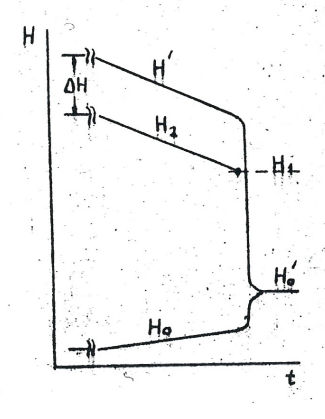
\includegraphics[width=0.45\textwidth]{fig_03.png}
\caption*{\textbf{Рис. 3.} Схема перехода кольцара в равновесное состояние
вследствие изотермической переконденсации}
\end{figure}

\subsubsection*{§2. Парадокс режима циркуляции}

Таким образом, сам по себе подъём жидкости в обводной трубке на уровень
$H > H_2$ представляет собой вполне тривиальное явление, легко объясняемое
законами элементарной физики и наблюдаемое экспериментально. Однако технически
нетрудно создать условия, когда поведение кольцара становится загадочным. А
именно, если
\begin{equation}
H_3 < H', \label{eq:2}
\end{equation}
то жидкость может возвращаться из обводной трубки в пространство над пористой
перегородкой самопроизвольно, самотёком, в результате чего в системе
возникнет циркуляция.

\begin{figure}[h]
\centering
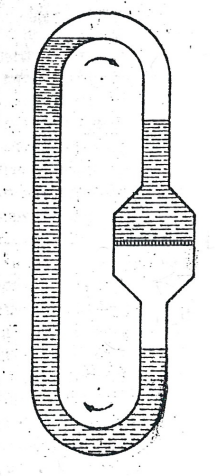
\includegraphics[width=0.45\textwidth]{fig_04.png}
\caption*{\textbf{Рис. 4.} Циркуляция жидкости в кольцаре Лазарева}
\end{figure}

Никнет циркуляция, и переход в равновесное состояние станет практически
невозможным при постоянных $\sigma$, $\theta$, $\rho$, $g$, $z$, определяющих
высоту дополнительного подъёма жидкости в обводной трубке $\Delta H$, а также
размерах самого сосуда. Получается так, что хотя все эти величины никак не
задаются законами сохранения, но именно от соотношения этих величин зависит
способность кольцара либо переходить в равновесное состояние, либо
функционировать в режиме, никак не предусмотренном равновесной термодинамикой
(рис.~4).

Более того, можно показать, что переход системы в равновесное состояние,
изображённое на рис.~3, вовсе не обязан происходить даже в том случае, если
при соблюдении условия~(1) условие~(2) не выполняется. Дело в том, что помимо
изотермической переконденсации жидкости между нижней поверхностью пористой
перегородки и дном сосуда, такой же процесс должен происходить и между
поверхностью жидкости в обводной трубке на высоте $H'$ и жидкостью, находящейся
над пористой перегородкой на высоте $H_2$. И если скорости этих процессов равны
(а они определяются не только давлением насыщенного пара, но и площадью
свободной поверхности жидкости, задаваемой размерами сосуда), то циркуляция
может продолжаться неопределённо долго.

Парадоксальность поведения кольцара Лазарева становится ещё более очевидной,
если учесть, что процессы испарения и конденсации сопровождаются тепловыми
эффектами. Это значит, что в системе, изотермической по определению, между
дном сосуда и пористой перегородкой должна самопроизвольно возникать
стационарная разность температур, то есть должно наблюдаться явление, которое
формально можно интерпретировать как явное нарушение второго начала
термодинамики.

%--- Страница 8--9 ---
\newpage

Необычность этого термодинамического парадокса заключается в его
обескураживающей очевидности: он разрешается как будто бы лишь в двух случаях
— либо в том, если пожертвовать элементарной физикой, отрицая существование
простого явления (капиллярного давления), либо в том, если пожертвовать
классической термодинамикой (допуская существимость «вечного двигателя»
второго рода). Вообще говоря, классическая физика не способна объяснить
квантовые явления типа сверхпроводимости (к которым не принято применять
законы термодинамики), а классическая термодинамика потерпела неудачу при
попытке объяснить явление жизни (которое считалось лишь термодинамикой
необратимых процессов). Но ведь кажется совершенно бесспорным, что кольцар
Лазарева не относится к квантовым системам и не требует для своего
существования подвода свободной энергии в какой-либо из известных форм.

В результате рассмотрение эффекта кольцара вызывает совершенно иррациональную,
чисто психологическую реакцию, когда поиск решения проблемы подменяется
упорным игнорированием как её самой, так и порождающих её фактов.

\subsubsection*{§3. Неквантовые системы с двумя состояниями}

Одна из характерных особенностей квантовых систем заключается в том, что они
могут одновременно находиться в двух различных стационарных состояниях.
Например, в молекулярном ионе водорода $\text{H}_2^+$ единственный электрон не
может быть связан только с одним из двух одинаковых протонов, а стремясь
принадлежать сразу им обоим, находится в непрерывном движении. В результате
между протонами, помимо сил обычного электростатического отталкивания,
возникает сила обменного взаимодействия, благодаря которой система обретает
устойчивость~[5]. Те же силы обменного взаимодействия между электронами
притягивают их в куперовские пары, благодаря чему близ абсолютного нуля
возникает сверхпроводимость. В известном смысле кольцо, по которому циркулирует
ток, вполне можно назвать кольцаром, потому что чисто внешне это явление тоже
не вписывается в круг явлений, допускаемых классической (обратимой)
термодинамикой.

Хорошо известные чисто квантовые эффекты (не только сверхпроводимость, но и
сверхтекучесть и туннелирование) не принято рассматривать с точки зрения
термодинамики по причинам скорее исторического, а не научного характера. А
именно, эти эффекты были сначала открыты экспериментально, а затем объяснены
теоретически, для чего пришлось использовать квантовомеханические представления,
принципиально отличающиеся от представлений классической физики и
принципиально игнорирующие существование второго начала термодинамики. В
соответствии с этим и все реальные объекты были разделены на две группы —
классические и квантовые, хотя совершенно очевидно, что подобное деление
совершенно условно, касается не самих объектов, а лишь способов их описания.
Поэтому если эффект сверхпроводимости наблюдается и объясняется (равно как и
другие квантовые эффекты) и наблюдается, а эффект кольцара наблюдается, но не
объясняется, то это вовсе не означает, что эффект кольцара реально не
существует и/или что его невозможно объяснить.

Приложение второго начала термодинамики к реальным системам требует, однако,
большой осторожности: оно даёт разумные результаты только в том случае, если
строго определено само понятие «система». В сильно неравновесных системах
явления, подобные циркуляции, вполне возможны; вопрос заключается лишь в том,
как долго они могут продолжаться. Если система изолирована, то продолжительность
циркуляции определяется запасом её свободной энергии и кинетикой процесса,
которая может быть сильно затруднённой из-за наличия высоких потенциальных
барьеров, особенно при низкой температуре. Если же система открытая, то
продолжительность циркуляции зависит от притока свободной энергии из
окружающей среды, который может быть значительным, а в пределе — практически
бесконечно большим. Если же мы не полностью понимаем, что что-то не знаем об
особенностях системы, то термодинамика позволяет судить о них лишь
проспективно по её наблюдаемому поведению.

Есть ли у сверхпроводящего кольца и кольцара Лазарева какие-либо общие
особенности помимо наблюдающейся циркуляции носителей вещества, не
сопровождающейся заметными диссипативными процессами?

Прежде всего, как сверхпроводящее кольцо, так и кольцар Лазарева,
представляют собой системы, явно далёкие от состояния термодинамического
равновесия, и применимость к ним законов обратимой термодинамики представляется
весьма сомнительной. Но это сходство не ограничивается. И в той, и в другой
системе циркуляция связана с существованием двух различных сил физического
взаимодействия (т.е. сил, имеющих различную физическую природу): в случае
сверхпроводящего кольца — сил кулоновского взаимодействия и обменных сил, а в
случае кольцара Лазарева — сил гравитации и межмолекулярных взаимодействий.
Результатом же совместного действия этих сил слу-

%--- Страница 10--11 ---
\newpage

жит возникновение двух различных стационарных состояний, что и оказывается
непосредственной причиной возникновения циркуляции.

Т.е. чисто феноменологически как квантовая, так и неквантовая системы
оказываются весьма схожими; различие заключается лишь в том, как это
интерпретировать, что считать причиной, а что следствием. Так, в квантовой
системе силы обменного взаимодействия считаются следствием существования двух
состояний, поскольку существование двух состояний изначально постулируется. В
неквантовой же системе причиной возникновения двух состояний оказываются силы,
заданные как физическая реальность.

Поэтому можно предположить, что любая (а не только квантовая) неравновесная
физическая система, в которой теоретически или экспериментально можно
обнаружить два стационарных состояния, должна вести себя подобно кольцару
Лазарева.

%--- Страница 10--11 (Глава II) ---
\newpage
\section*{ГЛАВА II}
\subsection*{Осмотический кольцар}

\subsubsection*{§1. Разрешение парадоксов}

В кольцаре Лазарева одно стационарное состояние определяется стремлением
системы прийти к равенству давления насыщенного пара над жидкостью, находящейся
в обводной трубке и над пористой перегородкой (это состояние может быть
достигнуто при условии $H' = H_2$), а другое — стремлением к равенству
гидростатического давления, создаваемого столбами жидкости слева и справа (это
состояние может быть достигнуто при условии $H' = H_4 - H_1$). Так как оба
указанных условия не могут одновременно выполняться, то в кольцаре возникает
циркуляция, которая прекращается или не возникает вовсе лишь в двух случаях:
если $H_0 = 0$ (когда не действуют силы поверхностного натяжения), или если
$H' = 0$ (когда отсутствует сила тяжести). Поэтому проблема заключается в том,
чтобы выяснить — каким образом кольцар может перейти в одно из двух равновесных
состояний.

Кольцар Лазарева интересен тем, что позволяет наблюдать экспериментально
эффект циркуляции; однако он неудобен как модель для выполнения количественных
оценок. Такой моделью может служить кольцар, в котором два состояния возникают
в результате осмоса.

Если в замкнутый кольцеобразный сосуд с полупроницаемой перегородкой поместить
с одной стороны чистый растворитель (например, воду), а с другой стороны
раствор какого-либо вещества, молекулы которого не способны проникать через
перегородку (например, сахарозы), то в соответствии с уравнением Вант-Гоффа
для идеальных растворов со стороны растворителя на раствор будет действовать
осмотическое давление
\[
P_\text{осм} = C_0^{(1)} RT,
\]
где $C_0^{(1)}$ — фактическая концентрация растворённого вещества близ
полупроницаемой перегородки, $R$ — газовая постоянная, а $T$ — абсолютная
температура. В результате условие гидростатического равновесия системы
определяется как
\begin{equation}
\bar{\rho} g H = C_0^{(1)} RT + \rho_2 g h, \label{eq:3}
\end{equation}
где $\bar{\rho}$ — средняя плотность раствора, $\rho_2$ — плотность
растворителя, $g$ — ускорение свободного падения, $H$ — высота уровня
раствора, а $h$ — высота уровня растворителя (рис.~5).

\begin{figure}[h]
\centering
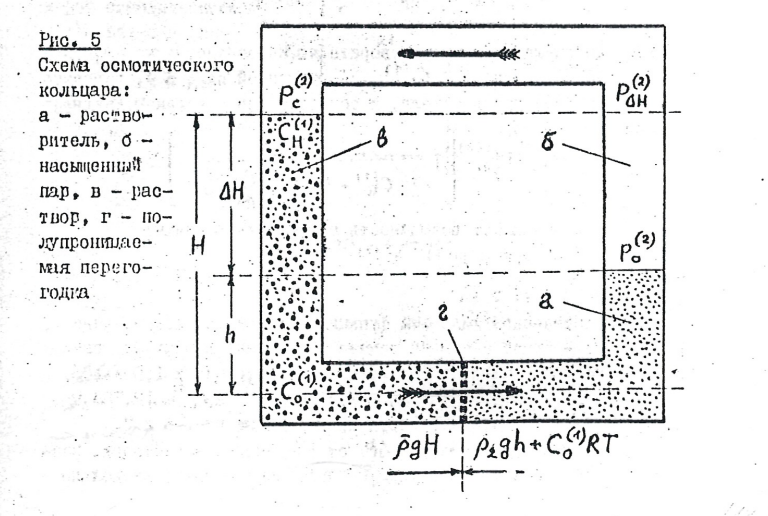
\includegraphics[width=0.45\textwidth]{fig_05.png}
\caption*{\textbf{Рис. 5.} Схема осмотического кольцара: а~— растворитель,
б~— насыщенный пар, в~— раствор, г~— полупроницаемая перегородка}
\end{figure}

В равновесных изотермических условиях под действием сил тяжести концентрация
растворённого вещества будет изменяться с высотой столба раствора по обычному
экспоненциальному закону, и поэтому на нулевом уровне, близ полупроницаемой
перегородки, она составит величину

%--- Страница 12--13 ---
\newpage

\begin{equation}
C_0^{(1)} = \frac{m_1 \rho_2 g (\rho_1 - \rho_2) H}{RT(m_1 \rho_2 + m_2 \rho_1)
\left(1 - e^{-\frac{m_1 g (\rho_1 - \rho_2) H}{\rho_1 RT}}\right)}, \label{eq:4}
\end{equation}
а на высоте $H$ концентрация раствора будет равна
\begin{equation}
C_H^{(1)} = \frac{m_1 \rho_2 g (\rho_1 - \rho_2) H}{RT(m_1 \rho_2 + m_2 \rho_1)
\left(e^{\frac{m_1 g (\rho_1 - \rho_2) H}{\rho_1 RT}} - 1\right)}. \label{eq:5}
\end{equation}
Здесь $\rho_1$ — плотность растворённого вещества, $m_1$ и $M_1$ — его масса
и молекулярный вес, а $m_2$ — масса растворителя, содержащегося в растворе.
Средняя же плотность раствора окажется равной
\begin{equation}
\bar{\rho} = \frac{\rho_1 \rho_2 (m_1 + m_2)}{m_2 \rho_1 + m_1 \rho_2}. \label{eq:6}
\end{equation}
Подставив~(\ref{eq:4}) и~(\ref{eq:6}) в~(\ref{eq:3}), получаем, что
\[
\Delta H = H - \frac{\rho_2(m_1+m_2)H}{m_1\rho_2+m_2\rho_1}
+ \frac{m_1(\rho_1-\rho_2)H}{(m_1\rho_2+m_2\rho_1)
\left(1 - e^{-\frac{m_1 g(\rho_1-\rho_2)H}{\rho_1 RT}}\right)}.
\]

Если давление насыщенного пара над чистым растворителем равно $P_0^{(2)}$, то
на высоте $H$ оно будет иметь величину
\[
P_{\Delta H}^{(2)} = P_0^{(2)}\, e^{-\frac{M_\text{в} g \Delta H}{RT}},
\]
где $M_\text{в}$ — молекулярный вес растворителя. Непосредственно же над
раствором с концентрацией $C_H^{(1)}$, определённой в~(\ref{eq:5}), давление
насыщенного пара растворителя, в соответствии с законом Рауля, составит
\[
P_c^{(2)} = P_0^{(2)} \left[1 - \frac{C_H^{(1)}}{C_H^{(1)} +
\frac{\rho_2}{M_1} \cdot \frac{M_\text{в} \rho_2}{\rho_1} C_H^{(1)}}\right].
\]
В результате возникает возможность определить величину
\[
\Delta P \approx P_c^{(2)} - P_{\Delta H}^{(2)}
\]
как функцию $C$, $H$ и $T$.

В аналитическом виде эта функция оказывается чрезвычайно громоздкой, в связи
с чем на основе справочных данных был выполнен расчёт для растворов сахарозы
с концентрациями 1,5 и 15\%. А именно, при 288~К (15$^{\circ}$С) $\rho_1 = 1{,}588$~г/см$^3$
и $P_0^{(2)} = 12{,}788$~мм рт.~ст. Результаты этого расчёта приведены на
рис.~6 и~7.

\begin{figure}[h]
\centering
% \includegraphics[width=0.5\textwidth]{fig6}
\caption*{\textbf{Рис. 6.} Зависимость $\Delta P$ от размеров осмотического
кольцара: а~— для 1,5\%-ного раствора сахарозы, б~— для 15\%-ного раствора
сахарозы}
\end{figure}

\begin{figure}[h]
\centering
% \includegraphics[width=0.45\textwidth]{fig7}
\caption*{\textbf{Рис. 7.} Зависимость $\Delta P$ от температуры системы:
а~— для 1,5\%-ного раствора сахарозы, б~— для 15\%-ного раствора сахарозы}
\end{figure}

Полученные зависимости $\Delta P$ от концентрации раствора, размера кольцара
$H$ и температуры $T$ позволяют сделать несколько выводов принципиального
характера.

1. Если $\Delta P \neq 0$, то в системе должна происходить циркуляция
растворителя (на рис.~5 её направление показано стрелками), подобная циркуляции
в кольцаре Лазарева.

2. Циркуляция растворителя прекратится лишь при выполнении хотя бы одного из
следующих условий: $C \to 0$, $H \to \infty$, $T \to 0$~К. Иначе говоря,
циркуляция невозможна лишь в истинно идеальной системе — имеющей бесконечно
большой размер и содержащей бесконечно разбавленный раствор, находящийся при
абсолютном нуле температуры.

3. То обстоятельство, что реальные системы отличаются от идеальных, не менее
существенно дела: так, циркуляция невозможна ниже температуры замерзания
растворителя, но это лишь сдвигает нижнюю границу осуществимости эффекта.

4. Как и в случае кольцара Лазарева, эффект возникает вследствие того, что
рассматриваемая система относится к классу систем с двумя стационарными
состояниями, одно из которых определяется условием равенства давлений
насыщенного пара на высоте $H$ над раствором и чистым растворителем, которые
в реальных условиях одновременно не выполняются.

5. Как и кольцар Лазарева, осмотический кольцар представляет собой систему,
явно далёкую от состояния термодинамического равновесия, достижение которого
сильно затруднено кинетически: полупроницаемая перегородка препятствует
смешению раствора с чистым растворителем, а летучесть растворённого вещества
может быть практически равна нулю. Вместе с тем, каким бы большим ни был
молекулярный вес растворённого вещества (это может быть, например, белок,
молекулы которого имеют размеры, существенно превышающие диаметр пор
перегородки), теоретически существует ненулевая вероятность того, что
растворённое вещество будет проникать через полупроницаемую перегородку, а
также испаряться из раствора. Иначе говоря, отличие величины $\Delta P$ от нуля
есть результат чисто кинетических затруднений.

Таким образом, совершенно очевидно, что теоретически продолжительность «жизни»
кольцара ограничена продолжительностью его существования в неравновесном
состоянии, однако практически она может быть сколь угодно большой — например,
сопоставимой с временем жизни Вселенной. В этом и заключается решение парадокса
кольцара: законы классической физики и обратимой термодинамики строго применимы
лишь к идеальным, равновесным системам, а кольцар представляет собой реальную,
неравновесную систему, и его поведение может быть корректно описано лишь
термодинамикой необратимых процессов.

\subsubsection*{§2. «Демон» кольцара}

Полупроницаемая перегородка, сортирующая молекулы по размерам, выполняет по
сути дела те же самые функции, что и «демон» Максвелла, сортирующий молекулы
по скоростям. И коль скоро такое устройство существует, следует уточнить, в
каком соотношении с законами термодинамики оно находится.

1. Если «демон» Максвелла работает, т.е. смещает термодинамическое равновесие,
при этом не потребляя свободной энергии, то мы имеем дело с нарушением второго
начала термодинамики.

2. Если «демон» Максвелла работает и при этом потребляет свободную энергию, но
ниоткуда её не получает, то мы имеем дело с нарушением первого начала
термодинамики.

3. Если «демон» Максвелла работает и при этом потребляет энергию, поступающую
из определённого источника, то никакого нарушения законов термодинамики не
происходит. Проблема заключается лишь в том, чтобы выяснить — находится ли
источник энергии внутри рассматриваемой системы, или же он расположен во
внешней среде. В первом случае работа «демона» будет сопровождаться
необратимой деградацией системы; во втором случае «демон» может работать
неопределённо долго, не вызывая внутри системы никаких изменений, поскольку
деградации будет подвергаться внешняя среда.

Поскольку циркуляция жидкости в кольцаре не только происходит (согласно
наблюдениям Лазарева), но и должна происходить (из-за существования двух
различных стационарных состояний), и в то же время у нас нет оснований
сомневаться в справедливости законов термодинамики, то поиск причин
возникновения эффекта должен сводиться к поиску источника энергии, питающего
«демона» кольцара.

Прежде всего обратим внимание на то, что свободная энергия, приводящая в
действие кольцар, имеет явно нетривиальную природу. Условия обычного
термодинамического равновесия осмотического кольцара и отсутствия циркуляции
соответствуют состоянию, когда на обе стороны полупроницаемой перегородки
находится раствор одинаковой концентрации. Как уже отмечалось, теоретически
существует ненулевая вероятность того, что молекулы растворённого вещества
способны проникать через полупроницаемую перегородку, а также испаряться с
поверхности раствора и конденсироваться на поверхности растворителя — т.е.
циркуляция растворителя в одном направлении (на рис.~5 против часовой стрелки)
может компенсироваться циркуляцией растворённого вещества в противоположном
направлении (по часовой стрелке). Однако, во-первых, вероятность такого
процесса может быть ничтожно малой, а во-вторых, это никак не означает, что
циркуляция от этого вовсе равна нулю — циркуляция от этого не прекращается,
а балансом сил, порождающих два стационарных состояния.

Совершенно очевидно, что кинетическую энергию молекул растворителя,
циркулирующих по замкнутому контуру кольцара, нельзя превратить в полезную
работу — например, поставив на пути потока турбину, поднимающую грузы. По
мере роста груза температура кольцара станет снижаться, и когда она достигнет
0~К, процесс циркуляции прекратится. После этого груз, опускаясь, превратит
свою потенциальную энергию, запасённую грузом, в тепло и вновь попытается
запустить кольцар.

%--- Страница 16--17 ---
\newpage

в тепло, в результате чего кольцар нагреется до первоначальной температуры.
И этот процесс изотермического превращения тепла в полезную работу можно,
по-видимому, повторять сколь угодно много раз — во всяком случае до тех пор,
пока кольцар продолжает оставаться в неравновесном состоянии.

Следовательно, каким бы образом мы не пытались изолировать кольцар от
обычных термодинамических контактов с внешней средой, он всё равно останется
принципиально открытой системой, в которую непрерывно поступает поток энергии
от источника высокого потенциала к источнику низкого потенциала. Этот поток
энергии, поддерживающий в стационарно-неравновесном состоянии как кольцар,
так и любые другие метастабильные структуры, имеет, скорее всего,
космофизическую природу, о чём свидетельствует обнаруженная связь между
флуктуациями мощности, развиваемой кольцаром Лазарева, и вариациями солнечной
активности Солнца. В этом космофизическом ключе следует рассматривать и
проблему существования «демона» Максвелла как особого термодинамического
устройства, обеспечивающего термодинамические контакты между всеми
неравновесными системами Вселенной.

\subsubsection*{§3. Кинетические признаки двух состояний}

Само по себе обнаружение циркуляции жидкости по замкнутому контуру не может
служить надёжным доказательством существования эффекта кольцара, поскольку
заранее неизвестно, как долго эта циркуляция будет продолжаться и не является
ли она тривиальным переходным процессом или не вызывается ли какими-либо
тривиальными внешними воздействиями. Такого рода доказательством может служить
лишь обнаружение способности системы находиться в двух различных стационарных
состояниях, поскольку в этом случае можно утверждать, что циркуляция должна
возникать совершенно неизбежно и \textbf{обязана} продолжаться сколь угодно
долго.

В осмотическом кольцаре, как и в кольцаре Лазарева, одно состояние
определяется стремлением системы к достижению равенства гидростатических
давлений, создаваемых столбами жидкости в сообщающихся сосудах; другое
состояние определяется условием равенства давлений насыщенного пара над
раствором и чистым растворителем. Чтобы привести систему в одно из таких
состояний, необходимо разомкнуть контур осмотического кольцара либо вверху,
либо внизу, и позволить системе достичь состояния динамического равновесия,
пока скорости потоков молекул растворителя (в жидкой

фазе или в парах) не станут одинаковы в обоих направлениях — слева направо и
справа налево.

До если после этого вновь замкнуть контур кольцара и при этом регистрировать
скорость и направление массопереноса растворителя, то обнаружится, что каждому
из двух различных стационарных состояний соответствует своя характерная
кинетика: в одном случае на плато будет наблюдаться плавный выход массопереноса
на плато, а в другом случае выход на то же самое плато будет происходить с
изменением направления массопереноса (рис.~8); при этом из-за того, что
жидкость обладает определённой инерцией, в самом начале процесса выхода
кольцара в режим циркуляции должны наблюдаться колебания скорости
массопереноса с характерными для данной конкретной системы периодами и
временами затухания.

\begin{figure}[h]
\centering
% \includegraphics[width=0.5\textwidth]{fig8}
\caption*{\textbf{Рис. 8.} Две кинетики перехода кольцара из двух различных
стационарных состояний в режим циркуляции. Пунктирной линией показаны
колебания, которые должны сопровождать скорость массопереноса на плато}
\end{figure}

Обнаружение двух таких кинетик и будет служить доказательством того, что в
системе могут существовать два различных стационарных состояния, в результате
чего жидкость в кольцаре не связана с каким-либо конкретным процессом и может
продолжаться неопределённо долго.

%--- Страница 18--19 (Глава III) ---
\newpage
\section*{ГЛАВА III}
\subsection*{Электрофизический кольцар}

\subsubsection*{§1. Постановка задачи}

Поскольку между движением жидкости по трубам и тока по проводам можно провести
определённую формальную аналогию, то имеет смысл рассмотреть электрофизический
аналог кольцара, в котором роль жидкости играют электроны проводимости двух
различных металлов, а роль полупроницаемой перегородки — полупроводник.
Будет ли в такой системе происходить циркуляция носителей заряда, подобная
циркуляции молекул жидкости в кольцаре Лазарева или осмотическом кольцаре?

Ответ на этот вопрос будет положительным, если в устройстве, схематически
изображённом на рис.~9, удастся обнаружить два различных стационарных состояния.

Если привести в соприкосновение два металла с различными работами выхода
электронов, то между этими металлами возникает т.н. контактная разность
потенциалов
\begin{equation}
\Delta\varphi_{12}' = -\frac{E_1 - E_2}{e}, \label{eq:7}
\end{equation}
где $E_1$ — работа выхода электрона из металла~1, $E_2$ — работа выхода
электрона из металла~2, а $e$ — заряд электрона. За счёт этой разности
потенциалов электроны могут совершать полезную работу, однако, нельзя: если
концы такого диполя замкнуть каким-либо проводником, то ме-

\begin{figure}[h]
\centering
% \includegraphics[width=0.45\textwidth]{fig9}
\caption*{\textbf{Рис. 9.} Схема электрофизического кольцара: а,~б~— металлы
с различными работами выхода электронов и концентрациями носителей заряда,
в~— полупроводник}
\end{figure}

жду ними и металлами 1 и 2 тоже возникнут контактные разности потенциалов,
причём их величины окажутся такими, что электрон, совершив полный оборот по
замкнутому контуру, не приобретёт никакой дополнительной энергии. Однако при
этом учитывается из вида, что движение тел (в том числе и электронов
проводимости) управляется не только энергией, но и силой.

Между тем, помимо контактной разности потенциалов $\Delta\varphi_{12}'$
(называемой первым потенциалом Вольта), между контактирующими металлами
возникает ещё и разность потенциалов $\Delta\varphi_{12}''$ (называемая вторым
потенциалом Вольта), определяемая различием концентраций носителей заряда
$n_{b1}$ и $n_{b2}$ в металлах 1 и 2:
\[
\Delta\varphi_{12}'' = \frac{kT}{e}\ln\frac{n_{b1}}{n_{b2}}.
\]
В свою очередь, в классическом приближении концентрация электронов проводимости
в металле можно считать равной
\[
n_b = N_A \mathcal{Z} e \frac{\rho}{A},
\]
где $N_A$ — число Авогадро, $\mathcal{Z}$ — валентность металла, $A$ — его
атомный вес и $\rho$ — плотность. Откуда
\begin{equation}
\Delta\varphi_{12}'' = \frac{kT}{e}\ln\frac{\mathcal{Z}_1 \rho_1 A_2}
{\mathcal{Z}_2 \rho_2 A_1}. \label{eq:8}
\end{equation}

Из выражений~(\ref{eq:7}) и~(\ref{eq:8}) следует, что величины $\Delta\varphi_{12}'$
и $\Delta\varphi_{12}''$ совершенно независимы друг от друга: одна из них
($\Delta\varphi_{12}'$) определяется взаимодействием электронов с кристаллической
решёткой металла (т.к. работа выхода отсчитывается от уровня Ферми), а другая
($\Delta\varphi_{12}''$) зависит от свойства атомов, образующих кристаллическую
решётку (их валентности, массы и способности взаимодействовать друг с другом).
Поэтому у разных металлов контактирующих пар $\Delta\varphi_{12}'$ и
$\Delta\varphi_{12}''$ могут иметь как одинаковые, так и противоположные знаки.
Например, для пары Zn--Ni вычисленные значения $\Delta\varphi_{12}' = +400$~мВ
и $\Delta\varphi_{12}'' = -11{,}7$~мВ, то для пары Be--Ag значения
$\Delta\varphi_{12}' = +400$~мВ и $\Delta\varphi_{12}'' = +35{,}7$~мВ. Это и
определяет способность системы, состоящей из двух контактирующих металлов,
находиться в двух различных стационарных состояниях — одном, определяемом
работой выхода электронов, и другом, определяемом концентрацией носителей
заряда.

Если сравнить осмотический кольцар с его электрофизическим аналогом, то мы
можем сделать вывод, что в электрофизической системе роль осмотического
давления выполняет разность потенциалов электронов с кристаллической решёткой
(определяемая работой выхода), а

%--- Страница 20--21 ---
\newpage

роль давления насыщенного пара — концентрация носителей заряда. Когда металлы
1 и 2, первоначально находящиеся при одном потенциале, соединяются друг с
другом проводником, то по нему начинает течь ток, направление которого
определяется соотношением работ выхода. После того, как между металлами
возникает разность потенциалов $\Delta\varphi_a'$, этот первичный ток должен
прекратиться, а работы выхода станут одинаковыми. Однако и в общем случае при
разности потенциалов $\Delta\varphi_a'$ равенство концентраций носителей заряда
в металлах 1 и 2 не будет достигнуто, и по проводнику должен пойти вторичный
ток, определяемый знаком и величиной $\Delta\varphi_a''$. В свою очередь, это
— следствие того, что первоначально равенство работ выхода нарушится, и по
проводнику вновь потечёт первичный ток — и т.д. Иначе говоря, два металла,
соединённых друг с другом проводником, находятся в динамическом равновесии,
определяемом разностью потенциалов $\Delta\varphi_a = \Delta\varphi_a' +
\Delta\varphi_a''$.

В устройстве, изображённом на рис.~9, должны происходить те же самые процессы
перераспределения зарядов. Однако в этом случае создаются условия, когда
вторичное перераспределение зарядов, определяемое разностью потенциалов
$\Delta\varphi_a''$, может происходить по замкнутому контуру. Это значит, что
в цепи электрофизического кольцара должна циркулировать величина и направление
которого определяется знаком и величиной $\Delta\varphi_a''$, а также
сопротивлением полупроводника. Поскольку $\Delta\varphi_a''$ имеет порядок
30~мВ, то в цепи с сопротивлением 100~МОм должен наблюдаться ток порядка
$\sim 10^{-10}$~А. Измерение такого тока представляет собой вполне разрешимую
экспериментальную задачу.

\subsubsection*{§2. Материалы, приборы и методы\footnote{В экспериментальной
части работы принимали участие А.И.Шаров, А.Ш.Гаяс, Я.И.Верцалмах,
Н.К.Невесский и В.А.Фёдоров.}}

Образцы для исследования готовились методом термического напыления в высоком
вакууме тонких слоёв (10 $\div$ 20~мкм) алюминия, серебра и бериллия (чистота
не менее 99,99\%) на противоположные стороны пластин (диаметром 30 $\div$ 40~мм,
толщиной 0,2 $\div$ 0,8~мм), вырезанных из монокристаллов фосфида галлия
($p$- и $n$-типа), а также $p/n$-переходов на основе фосфида галлия. Нумерация
образцов, их структура и качественные результаты испытаний на способность
генерировать ток приведены в следующей таблице:

\begin{table}[h]
\centering
\begin{tabular}{|l|c|c|c|}
\hline
& Структура образца & Толщина п/п частицы & Эффект \\
\hline
Образец 1 & $\text{Ag-}p[\text{GaP}]\text{-Al}$ & 0,8~мм & --- \\
Образец 2 & ${}^{\oplus}\text{Ag-}n[\text{GaP}]\text{-Al}^{\ominus}$ & ---~"--- & + \\
Образец 3 & $\text{Ag-}p[\text{GaP}]\text{n-Al}$ & ---~"--- & --- \\
Образец 4 & ${}^{\oplus}\text{Ag-}n[\text{GaP}]\text{p-Al}^{\ominus}$ & ---~"--- & + \\
Образец 5 & $\text{Ag-}n[\text{InP}]\text{-Al}$ & ---~"--- & --- \\
Образец 6 & $n[\text{GaP}]n$ (контроль) & ---~"--- & --- \\
Образец 7 & ${}^{\oplus}\text{Ag-}n[\text{GaP}]\text{-Al}^{\ominus}$ & 0,2~мм & + \\
Образец 8 & $\text{Ag-}n[\text{GaP}]\text{n-Be}$ & ---~"--- & + \\
\hline
\end{tabular}
\end{table}

Предварительные качественные испытания образцов были выполнены при помощи
зеркального гальванометра. При цене деления 1~нА замыкание цепи, в которую
были включены образцы 2 $\div$ 4, приводило к отклонению светового зайчика на
3 $\div$ 5 делений, причём изменение полярности включения образца приводило к
изменению направления тока; образцы 1,3,5 и~6 (контроль) тока не генерировали.

Для всех последующих количественных исследований использовался
электрометрический вольтметр У7-45 (производство Минского завода им.
В.И.Ленина) с разрешающей способностью, позволяющей измерять токи в диапазоне
от $10^{-9}$ до $10^{-17}$~А. Согласно паспортным данным, дрейф нулевой точки
прибора не превышает $\cdot 10^{-17}$~А за 24~ч непрерывной работы;
среднеквадратичная амплитуда шума на аналоговом выходе составляет не более
$2{,}0 \cdot 10^{-16}$~А. Измерения производились на поддиапазонах $10^{-9}
\div 10^{-10}$~А и в трёх различных режимах:
\begin{itemize}
  \item с использованием цифровой памяти и памяти прибора;
  \item с помощью самописца, подключённого к аналоговому выходу;
  \item с помощью ЦВМ, подключённой к цифровому выходу АЦП.
\end{itemize}
Исследуемые образцы помещались либо непосредственно в закрытой измерительной
камере прибора и включались в цепь с помощью двух медных электродов (диаметр
50~мм, толщина 5~мм) с посеребрёнными

%--- Страница 22--23 ---
\newpage

контактирующими поверхностями (рис.~10), либо в выносной экранированной камере
(рис.~11).

Вольтамперные характеристики образцов измерялись по схеме, изображённой на
рис.~12.

\begin{figure}[h]
\centering
% \includegraphics[width=0.45\textwidth]{fig10}
\caption*{\textbf{Рис. 10.} Схема размещения образцов в измерительной камере
прибора: а~— камера, б~— медные электроды, в~— образец, г~— полиэтиленовая
изоляция}
\end{figure}

\begin{figure}[h]
\centering
% \includegraphics[width=0.45\textwidth]{fig11}
\caption*{\textbf{Рис. 11.} Схема размещения образцов в выносной камере:
а~— пермаллоевый экран, б~— медные электроды, в~— образец, г~— тефлоновая
изоляция, д~— экранированный коаксиальный кабель}
\end{figure}

\begin{figure}[h]
\centering
% \includegraphics[width=0.35\textwidth]{fig12}
\caption*{\textbf{Рис. 12.} Схема измерения вольтамперных характеристик:
а~— образец, б~— сопротивление нагрузки ($0{,}1 \div 100$~МОм;
$E_n = 0{,}1 \div 29$~В, $U_n = E_n - U_{RH}$, $J = U_{RH}/R_H$)}
\end{figure}

\subsubsection*{§3. Результаты экспериментов и обсуждение результатов}

Результаты измерения вольтамперных характеристик образцов подтверждают
включённые выше результаты качественных испытаний и позволяют выявить их общие
свойства (рис.~13).

\begin{figure}[h]
\centering
% \includegraphics[width=0.6\textwidth]{fig13}
\caption*{\textbf{Рис. 13.} Вольтамперные характеристики различных образцов:
образцы 1, 5 и~6 (т.е. бimetalлические системы на основе фосфида галлия $p$-типа
и $n$-типа, а также контрольный образец без биметаллического покрытия) не дают
эффекта генерации тока и имеют обычные линейные вольтамперные характеристики;
образец~3 не даёт эффекта генерации тока, но имеет ВАХ диода и не генерирует
тока, но образцы 2 и~4 имеют асимметричные ВАХ, проходящие через область
отрицательного сопротивления}
\end{figure}

%--- Страница 24--25 ---
\newpage

характеристики, в то время как вольтамперные характеристики образцов 2, 3 и~4
нелинейны. Но нелинейность образца~3 существенно отличается от нелинейности
образцов 2 и~4: образец~3, как и образцы 1, 5 и~6, не генерирует тока и его
вольтамперная характеристика имеет вид, характерный для обычных линий
вольтамперных характеристик, она проходит через нуль и реа-

ко асимметрична. В отличие от этого, вольтамперные характеристики образцов 2
и~4 симметричны, но не проходят через область отрицательного сопротивления,
т.е. служат активными источниками тока. Кроме того, образец~4 (с которым
производились все последующие эксперименты) проявляет ещё одну интересную
аномалию, требующую дополнительного исследования: в нём проявляется своеобразный
эффект «памяти» (рис.~14).

\begin{figure}[h]
\centering
% \includegraphics[width=0.5\textwidth]{fig14}
\caption*{\textbf{Рис. 14.} Гистерезис явления, наблюдаемого в образце~4
(сплошными линиями указаны средние значения $U_n$): а~— каждая точка
представляет собой среднее из 100 отсчётов, выполненных за 10~сек.; б~—
каждая точка представляет собой среднее из 100 отсчётов, выполненных за 90~сек.}
\end{figure}

Образцы 2 и~3 отличаются друг от друга только ориентацией разноимённо
заряженных металлов (серебра и алюминия) относительно одного и того же $p/n$
перехода; существенное различие на вольтамперных характеристиках можно
приписать тому, что в образце~3 ориентация зарядов способствует увеличению
сопротивления двойного электрического слоя на $p/n$-переходе, а в образце~2 —
его уменьшению. Для пары серебро -- алюминий рассчитанное значение
$\Delta\varphi_{12}''$ составляет примерно $-28$~мВ; регистрируемое напряжение
тока, генерируемого образцом~2, как раз и свидетельствует о том, что серебро
несёт отрицательный, а алюминий — положительный заряды.

В образце~4 $p/n$-переход отсутствует вовсе; тем не менее, его вольтамперная
характеристика оказывается похожей на вольтамперную характеристику образца~2,
а не образцов 1, 3, 5 и~6. При этом образцы 2 и~4 генерируют ток порядка
$10^{-10} \div 10^{-11}$~А и имеют э.д.с. порядка $I \div 100$~мВ, т.е.
близкую по величине $\Delta\varphi_{12}''$.

Вообще говоря, причиной возникновения э.д.с. такого порядка могут служить
некоторые тривиальные факторы.

1. \underline{Различие температур электродов, соприкасающихся с различными
сторонами образца}. Действительно, генерируемый ток меняется с температурой
образца (рис.~15); однако этот эффект является, скорее всего,

\begin{figure}[h]
\centering
% \includegraphics[width=0.4\textwidth]{fig15}
\caption*{\textbf{Рис. 15.} Зависимость тока, генерируемого образцом~4, от
температуры в измерительной камере}
\end{figure}

%--- Страница 26--27 ---
\newpage

следствием увеличения с температурой сопротивления полупроводника при
практически постоянной э.д.с., потому что термоэлектродвижущая сила порядка
1~нВ может возникать при разности температур порядка $30^{\circ}$С; такой
градиент не мог возникать в условиях опыта (тем более, что зазор между
массивными медными электродами составлял $\sim 1$~мм). Более того, этот фактор
отклоняется по той причине, что переворот образца на $180^{\circ}$ (т.е.
сохранение полярности подключения электродов) приводит к изменению направления
тока на противоположное, в то время как если бы причиной возникновения тока
был градиент температур, то такого изменения бы не произошло.

2. \underline{Физико-химические процессы, происходящие при старении образцов}.
Действительно, такие процессы способны, в принципе, приводить к возникновению
э.д.с. Однако в этом случае образцы вели бы себя как обычные электрохимические
элементы, а не как системы с двумя стационарными состояниями (см. гл.~II, §3).
А именно, если металлы, нанесённые на поверхность полупроводника, связаны с
фазами кристаллической решётки, то в этом случае образцы оказываются
асимметричными, и работа выхода электронов — различными (состояние~1); если
же эти металлы накоротко замкнуть проводником, то работа выхода электронов
стремится стать одинаковой (состояние~2). Включение в измерительную цепь
образцов, подготовленных подобным образом, должно сопровождаться двумя
различными кинетиками тока на плато (ср. рис.~8); включение в измерительную
цепь обычного электрохимического элемента не может давать подобного эффекта.
При включении в измерительную цепь образца~4 как раз и удалось наблюдать две
отчётливые различающиеся и хорошо воспроизводимые кинетики (рис.~16), что
однозначно указывает на то, что эта система представляет собой настоящий
электрофизический кольцар. При этом, как и следовало

\begin{figure}[h]
\centering
% \includegraphics[width=0.45\textwidth]{fig16}
\caption*{\textbf{Рис. 16.} Две различные кинетики выхода тока на плато:
а~— из состояния~1, б~— из состояния~2 ($\tau \sim 40$~сек.)}
\end{figure}

ожидать, выход тока на плато сопровождается затухающими гармоническими
колебаниями с амплитудами, периодами и временем затухания, характерными для
каждого конкретного образца (рис.~17). Точно так же колебания возникали и в
том случае, если в измерительной цепи возбуждался импульсный ток (рис.~18),
что указывает на то, что период колебаний и время их затухания определяются
$RC$-характеристиками образцов.

3. \underline{Влияние внешних естественных и/или искусственных электромагнитных
полей}. Действительно, затухающие гармонические колебания, изображённые на
рис.~18, возникали в измерительной цепи в результате воздействия на
индуктивность измерительной камеры импульсного магни-

\begin{figure}[h]
\centering
% \includegraphics[width=0.45\textwidth]{fig17}
\caption*{\textbf{Рис. 17.} Кинетика выхода тока на плато у различных
образцов: а~— образец~7 ($\tau \sim 15$~сек.), б~— образец~8 ($\tau \sim 25$~сек.)}
\end{figure}

\begin{figure}[h]
\centering
% \includegraphics[width=0.45\textwidth]{fig18}
\caption*{\textbf{Рис. 18.} Появление затухающих гармонических колебаний после
возбуждения импульсного тока в измерительной цепи: а~— при образце~4
($\tau \sim 40$~сек.), б~— при образце~7 ($\tau \sim 15$~сек.), в~— при
образце~8 ($\tau \sim 25$~сек.); момент возбуждения импульсного тока отмечен
стрелкой}
\end{figure}

%--- Страница 28--29 ---
\newpage

ного поля (постоянный магнит с напряжённостью $\sim 100$~Э быстро проносился
над измерительной камерой с помощью и не образцом или с \textbf{подключённым
к прибору образцом, находящимся в выносной экранированной камере}). Магнитные
поля, амплитуда колебаний которых не превышает $10^{-2}$~Э, способны, в
принципе, возбуждать в измерительной цепи затухающие гармонические колебания
тока с амплитудой до $10^{-12}$~А (в случае образца~7) и до $10^{-14}$~А (в
случае образца~4), но не генерировать постоянный ток, поскольку образец~4, не
обладающий выпрямляющими свойствами, судя по его вольтамперной характеристике
(см. рис.~13); более того, именно в случае образца~4, генерирующего
максимальный ток, измерительная цепь оказывается наименее восприимчивой к
воздействию импульсного магнитного поля. Что не касается высокочастотных
радиоизлучений, то они достаточно хорошо экранируются стенками измерительной
камеры, что подтверждается высокой стабильностью показаний прибора при
измерениях на поддиапазоне $10^{-15}$~А; стенки измерительной камеры (клетка
Фарадея) экранируют измерительную цепь и образцы и от действия
электростатических полей.

Таким образом, вполне можно считать вполне доказанным, что наблюдаемый
электрофизический эффект (циркуляция тока по незамкнутому электрофизическому
кольцу при комнатной температуре) представляет собой истинный эффект кольцара;
возможно, что он как-то связан с известным эффектом высокотемпературной
сверхпроводимости, поскольку высокотемпературные сверхпроводники, как и
электрофизический кольцар, имеют сложную многокомпонентную структуру.

Электрофизический кольцар имеет ещё одно свойство, отличающее его в один ряд
с кольцаром Лазарева: в нём наблюдаются флуктуации, имеющие (по крайней мере,
частично) явно космофизическое происхождение. Изучение подобных флуктуаций и
была посвящена значительная часть экспериментов, посвящённых электрофизическому
кольцару.

Ток, генерируемый различными образцами, различается не только по величине, но
и по характеру флуктуаций. Так, образец~4 генерирует самый большой ток с самой
малой амплитудой флуктуаций; такой же ток, генерируемый образцом~7, имеет
меньшую амплитуду флуктуаций; флуктуации тока образца~8 тоже значительны, но
не приводят к изменению знака эффекта (рис.~19). Так как образец~4

\begin{figure}[h]
\centering
% \includegraphics[width=0.6\textwidth]{fig19}
\caption*{\textbf{Рис. 19.} Флуктуации тока, генерируемого различными образцами
при постоянной интегрировании 10~сек.: а~— образец~4, б~— образец~7,
в~— образец~8}
\end{figure}

\begin{figure}[h]
\centering
% \includegraphics[width=0.6\textwidth]{fig20}
\caption*{\textbf{Рис. 20.} Флуктуации тока, генерируемого образцом~4: сигнал
(вверху), спектр мощности после компенсации постоянной составляющей (внизу)}
\end{figure}

%--- Страница 30--31 ---
\newpage

генерирует самый большой ток (т.е. демонстрирует отчётливый эффект кольцара),
то именно он в дальнейшем использовался для изучения флуктуаций.

Прежде всего, эти флуктуации имеют характер неравновесного низкочастотного
шума типа $1/f$ с бесконечными дисперсиями. Если компенсировать постоянную
составляющую тока, генерируемого кольцаром (на основе образца~4), то в
спектре мощности (на основе образца~4) наблюдаются разрядки, но отчётливо
выражены максимумы в области $0{,}4 \div 0{,}8$~Гц (рис.~20). В области
более высоких частот наблюдается только обычный

тепловой шум с малой амплитудой (хотя, возможно, что высокочастотные флуктуации
$1/f$-типа просто фильтруются измерительной цепью с большой постоянной
времени), в связи с чем основное внимание было обращено на низкочастотную
область спектра (постоянная составляющая тока, генерируемого кольцаром, может
рассматриваться как флуктуации с частотой $f \to 0$).

С этой целью была выполнена длительная серия измерений тока, генерируемого
образцом~4 (всего 72~сут. непрерывных наблюдений); отсчёты делались каждые
15~мин. с постоянной интегрирования 100~сек. Типичный ход изменений тока в
одно и то же время суток в разные дни приведён на рис.~21. Он отличает их не
только значительная амплитуда флуктуаций (приборная ошибка измерения тока не
превышает на соответствующем поддиапазоне $\sim 3 \cdot 10^{-12}$~А), а также
то, что среднее значение тока может как оставаться постоянным, так и резко
меняться при практически постоянной температуре ($\pm 0{,}2^{\circ}$С), т.е.
когда температурный дрейф (см. рис.~15) не мог превышать $\sim 15$~от
измеренной величины, т.е. $\sim 2 \cdot 10^{-12}$~А. Такие изменения носят
нередко случайный характер (рис.~22), вследствие чего дальнейшему анализу

\begin{figure}[h]
\centering
% \includegraphics[width=0.6\textwidth]{fig21}
\caption*{\textbf{Рис. 21.} Флуктуации тока, генерируемого образцом~4, в разные
дни в одно и то же время суток (LT — местное время): а~— 1.06.92~г.,
б~— 2.06.92~г., в~— 3.06.92~г.}
\end{figure}

\begin{figure}[h]
\centering
% \includegraphics[width=0.35\textwidth]{fig22}
\caption*{\textbf{Рис. 22.} Флуктуации тока, генерируемого образцом~4,
непрерывно на протяжении 9~суток. Отсчёты проводились каждые 9~суток.
Отчётливо просматривается периодичность с периодом $\sim 7$~сут. (среднее
значение тока с первого по первый сут. составляет $\sim 7$~сут.)}
\end{figure}

%--- Страница 32--33 ---
\newpage

были подвергнуты флуктуации низкой частоты.

Флуктуации среднесуточных значений тока (рис.~23) также имеют квазипериодический
характер при значительной амплитуде (периоды $10^{-10}$~А); лишь отдельные
выбросы (например, 21-й день) можно приписать влиянию температурного фактора,
в целом значимой связи флуктуаций тока с изменениями температуры в измерительной
цепи не наблюдается. Однако ритмика флуктуаций тока (наличие в них достаточно
выраженного периода $\sim 33$~сут.) поразительным образом совпадает с ритмикой
изменений солнечной активности Солнца (период $\sim 32$~сут.), происходящих во
время эксперимента, а также имеет некоторые общие черты с ритмикой вариаций
общепланетарной геомагнитной возмущённости (рис.~21).

Предварительное суждение о причинах и механизме возникновения общих ритмов
может дать функция взаимной корреляции флуктуаций тока, явлений изменений
солнечной активности и геомагнитной возмущённости (рис.~25). Из их совместного
рассмотрения можно сделать следующие выводы.

1. Флуктуации тока в электрофизическом кольцаре явно связаны с вариациями
солнечной активности и переносятся на Землю солнечным

\begin{figure}[h]
\centering
% \includegraphics[width=0.55\textwidth]{fig23}
\caption*{\textbf{Рис. 23.} Флуктуации среднесуточных значений тока,
генерируемого образцом~4. Участки, обозначенные цифрами I и~II, были
использованы для обработки методом наложенных эпох (см. ниже рис.~27)}
\end{figure}

\begin{figure}[h]
\centering
% \includegraphics[width=0.45\textwidth]{fig24}
\caption*{\textbf{Рис. 24.} Автокорреляционные функции: а~— флуктуаций тока,
генерируемого образцом~4, б~— изменения солнечной активности (международные
$R_i$-индексы), в~— вариаций общепланетарной геомагнитной возмущённости
($A_p$-индексы). Периоды $32^d$, $33^d$ и $21^d$ превышают уровень
достоверности $36^d$ ($p < 0{,}005$)}
\end{figure}

\begin{figure}[h]
\centering
% \includegraphics[width=0.45\textwidth]{fig25}
\caption*{\textbf{Рис. 25.} Функция взаимной корреляции: а~— флуктуаций тока
и $R_i$-индексов (солнечной активности), б~— флуктуаций тока и $A_p$-индексов
(геомагнитной возмущённости), в~— $A_p$-индексов и $R_i$-индексов.
Зависимость флуктуаций тока и геомагнитной возмущённости от активности
Солнца имеет одинаковый характер, но прямая связь флуктуаций тока с
геомагнитной возмущённостью отсутствует ($r_c = 0$ при $0^d$)}
\end{figure}

%--- Страница 34--35 ---
\newpage

ветром (запаздывание на $\sim 5$~сут., практически равное запаздыванию
возмущённости магнитосферы Земли, вызываемой этим важнейшим
космофизическим фактором, ответственным также за связь Солнце -- биосфера
[6]).

2. Вариации возмущённости геомагнитного поля не оказывают непосредственного
влияния на флуктуации тока в электрофизическом кольцаре, а связаны с ними
лишь косвенно, поскольку вызываются одним и тем же космофизическим фактором
— солнечным ветром (но, возможно, его различными составляющими [7]).

3. Имеется некоторый намёк на существование корреляции между флуктуациями
тока и солнечной активностью без сдвига по фазе (период на функции $\gamma_c$
при $0^d$), т.е. о наличии фактора, осуществляющего быструю (в сравнении с
солнечным ветром) солнечно-земную связь (ср. [8,~9]).

Полученные результаты представляются достаточно странными и требуют ответа на
вопрос: какова всё-таки природа космофизического фактора, вызывающего флуктуации
тока в электрофизическом кольцаре? Необычность этого фактора усугубляется ещё
двумя наблюдениями. Во-первых, попытки избавиться от флуктуаций тока
дополнительной экранировкой образца не дали заметного результата (рис.~26).
Во-вторых, когда методом наложенных эпох из флуктуаций тока были выделены
регулярные суточные компоненты (рис.~27), то они оказались поразительно
похожими на регулярные суточные изменения азимута $\Theta$ большой оси

\begin{figure}[h]
\centering
% \includegraphics[width=0.45\textwidth]{fig26}
\caption*{\textbf{Рис. 26.} Результаты наблюдений флуктуаций тока, генерируемого
образцом~4 в выносной измерительной камере: а~— без защиты от внешних
воздействий, б~— в заземлённом пермаллоевом экране (см. рис.~11)}
\end{figure}

\begin{figure}[h]
\centering
% \includegraphics[width=0.45\textwidth]{fig27}
\caption*{\textbf{Рис. 27.} Регулярные суточные компоненты флуктуаций тока,
генерируемого образцом~4 (см. рис.~23), и изменения азимута большой оси
поляризационного эллипса РеЗ (обсерватория Боров, заимствовано из [10])}
\end{figure}

%--- Страница 36--37 ---
\newpage

эллипса поляризации микроволнового геомагнитного поля РеЗ (т.е. его
ориентации относительно земного меридиана), причём в этом случае никаких
фазовых сдвигов не наблюдается.

Микроволновое поле РеЗ, частота которого лежит в области $0{,}02 \div 0{,}1$~Гц
(ср. рис.~20), часто рассматривается как непосредственный фактор, ответственный
за наибольшие связи Солнце -- биосфера [10]; однако этот фактор слишком слаб
для того, чтобы вызывать заметные физические эффекты. Поэтому сходство и
\textbf{совпадение по фазе суточных компонент флуктуаций тока электрофизического
кольцара и величины $\Theta$} (не имеющей прямой физической интерпретации
геомагнитного поля) может быть лишь следствием того, что они имеют общее
космофизическое происхождение.

По-видимому, непосредственной причиной флуктуаций тока, генерируемого
электрофизическим кольцаром, служат изменения работы выхода электронов, т.е.
флуктуации высоты потенциальных барьеров; в свою очередь, эти энергетические
флуктуации могут служить общей причиной возникновения т.н. макрофлуктуаций в
системах различной природы [3,~4]. В случае электрофизического кольцара
изменения работы выхода электронов должны приводить к соответствующему
перераспределению носителей заряда между двумя различными электрическими
слоями, и, следовательно, к возникновению флуктуаций основного тока в
измерительной цепи [11]. Такое устройство может считаться весьма перспективным
объектом для систематического изучения макрофлуктуаций, поскольку в этом случае
высокой сигнал представляет собой прямое следствие порождающей его причины и
требует лишь соответствующего усиления (рис.~28).

\begin{figure}[h]
\centering
% \includegraphics[width=0.45\textwidth]{fig28}
\caption*{\textbf{Рис. 28.} Вероятные изменения ВАХ образцов при флуктуациях
тока в электрофизических кольцарах: а~— изменения ВАХ между типом диода и
активным источником тока, б~— изменения ВАХ между типом активного источника
тока и линейным сопротивлением (см. рис.~13)}
\end{figure}

\newpage
\section*{ВЫВОДЫ}

Эффект кольцара (особенно в его электрофизическом варианте) заслуживает самого
тщательного теоретического и экспериментального исследования не только из-за
возможных следствий фундаментального характера, но и из-за результатов,
способных иметь высокую практическую ценность.

Разумеется, вряд ли можно надеяться на то, что кольцар способен служить
источником полезной энергии: развиваемая им мощность (порядка $10^{-10} \div
10^{-12}$~Вт) слишком мала и вряд ли в ближайшее время может быть значительно
повышена путём даже самой плотной упаковки его структурных элементов. Однако
для такой мощности вполне достаточно для того, чтобы на базе эффекта
электрофизического кольцара создать принципиально новые нелинейные элементы
микроэлектроники, способные моделировать процессы возбуждения и торможения,
происходящие в головном мозге. Нельзя исключить и возможности того, что
изучение эффекта электрофизического кольцара способно привести к созданию новых
высокотемпературных сверхпроводников. Наиболее же реальные перспективы
использования электрофизических кольцаров заключаются в создании на их основе
приборов, позволяющих изучать солнечно-земные связи с целью использования
получаемой информации для прогнозирования гелиогеофизических и гелиобиологических
событий экстремального характера, а также служить основой для разработки
принципиально новых средств связи.

%--- Страница 37--38 (Литература) ---
\newpage
\section*{ЛИТЕРАТУРА}

\begin{enumerate}
\item Жвирблис В.Е. «Кольцар» Лазарева: первый пример искусственной динамической
диссипативной структуры. Препринт № 1 МНЦ «ВЕНТ». М., 1991.

\item Пригожин И., Стенгерс И. Порядок из хаоса. М.: Прогресс, 1986.

\item Удальцова Н.В., Коломбет В.А., Шноль С.Э. Возможная космофизическая
обусловленность макрофлуктуаций в процессах различной природы. Пущино, 1987.

\item Владимирский Б.М. Макроскопические флуктуации, солнечно-земные связи и
методические проблемы точных измерений. Известия Крымской астрофизической
обсерватории, 1990, т.~82, с.~161--172.

\item Фейнман Р., Лейтон Р., Сэндс М. Фейнмановские лекции по физике.
М.: Мир, 1978, т.~8--9, с.~175--183.

\item Сидякин В.Г., Темурьянц Н.А., Макеев В.Б., Владимирский Б.М.
Космическая экология. Киев, Наукова думка, 1985.

\item Жвирблис В.Е. О воспроизводимости гелиобиологических экспериментов.
В кн.: Проблемы космической биологии, т.~65. Биофизические и клинические
аспекты гелиобиологии. Л.: Наука, 1989, с.~145--160.

\item Аджиев А.Г., Пулач А.Ф. К вопросу о возможности обнаружения торсионных
полей астрономическими методами. Препринт № 25 МНЦ «ВЕНТ». М., 1992.

\item Козырев Н.А. Линейная или несимметричная механика в линейном приближении.
Пулково, 1958.

\item Темурьянц Н.А., Владимирский Б.М., Тишкин О.Г. Сверхнизкочастотные
электромагнитные сигналы в биологическом мире. Киев, Наукова думка, 1992,
с.~109.

\item Жвирблис В.Е. Устройство для регистрации флуктуаций работы выхода
электронов. Патент Российской Федерации (заявка № 5020194/25 от 21.02.92~г.).
\end{enumerate}

%--- Страница 38 (Оглавление) ---
\newpage
\section*{ОГЛАВЛЕНИЕ}

\begin{tabbing}
Введение \dotfill 3 \\
Глава I. Кольцар Лазарева \dotfill 4 \\
Глава II. Осмотический кольцар \dotfill 10 \\
Глава III. Электрофизический кольцар \dotfill 18 \\
Выводы \dotfill 37 \\
\end{tabbing}

\vfill
\begin{flushleft}
\textbf{Жвирблис Вячеслав Евгеньевич}

\medskip
Феноменологическое описание и экспериментальное исследование некоторых кольцаров

\medskip
Препринт Межотраслевого научно-технического центра\\
венчурных нетрадиционных технологий (МНЦ «ВЕНТ»)

\medskip
Москва 125190, а/я 214
\end{flushleft}

\begin{flushright}
Подписано к печати 19.01.93~г.\\
Печ. л. 2,4.\\
Уч.-изд. л. 1,68.\\
Тираж 300 экз.\\
Цена договорная.
\end{flushright}

\end{document}
